\noindent{\Huge\scshape Л}{\LARGE\scshape ингвистика}\\
\rule[0.5\baselineskip]{\textwidth}{1pt}

\vspace{0\baselineskip}

% \begin{compactenum}
% \setlength\itemsep{-0.25em}
%     \item[31.]
\subsection*{Задание 31.}
    \textit{Дэвид Петерсон – американский писатель, художник, создатель искусственных языков для фильмов и сериалов, в том числе дотракийского и валирийского языков (сериал «Игра Престолов»). Петерсон часто выступает с открытыми лекциями в университетах, где рассказывает о процессе придумывания новых языков. В частности, на лекции в офисе Google он рассказывал о языках в сериале «Defiance» \url{https://youtu.be/Z50T-tslrgs}. Ниже приводится сокращенный фрагмент (19:10 – 28:35) его лекции, переведённый на русский язык.}
    
    В сериале «Defiance» есть несколько инопланетных рас. Индогены (Indogenes) — обладатели всех современных технологий. Их тела модифицированы с помощью имплантов. Каститанцы (Castithans) в прошлом завоевали планету ирасиентов (Irathient). Сейчас эти две расы равны, но между ними присутствует напряжение.
    
    Мне нужно было перевести несколько реплик из сценария на язык ирасиентов.  Вот эта фраза: \textit{«Именно так Кастис убил нас в Великой Диаспоре. Пещеры заполнены газообразным хлором».}
    
    Обратим внимание на словосочетание «газообразный хлор». В языке ирасиентов нет такого слова, поэтому его нужно заимствовать из языка высокотехнологичных индогенов — индоджиснена. 
    
    Письменность в языке индоджиснен апостериорная: индогены создали новую систему письма благодаря трансформациям в своих руках. В их письменности есть глифы, каждый глиф в языке — двойной шестиугольник. 
    
    Это их система счисления по основанию $7$.
    
    \begin{center}
    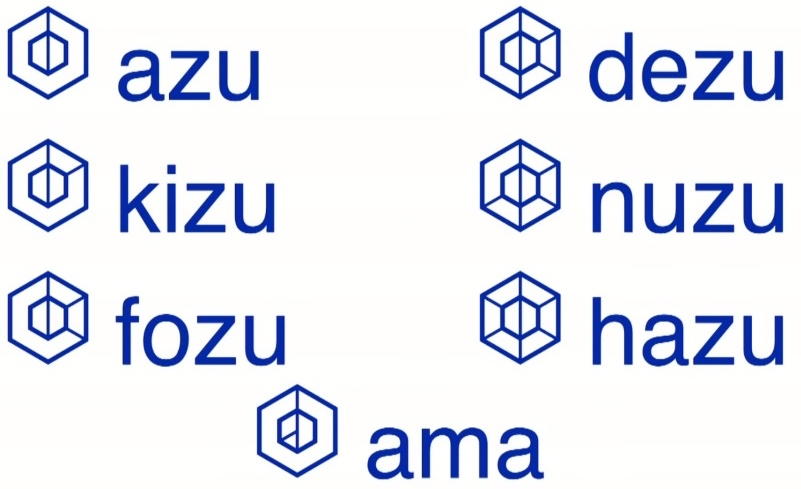
\includegraphics[scale=0.2]{lingua/image1-17.jpeg}
    \end{center}
    
    В каждой новой цифре добавляется палочка и мы получаем azu, kizu, fozu, dezu, nuzu, hazu, это $1, 2, 3, 4, 5, 6$. Затем меняется суффикс и получается ama — $7$. Я начал с этой системы, когда мне нужно было найти слова для элементов периодической системы элементов. Я решил, что они изобрели кодифицированную систему для соотнесения с химическими элементами. Они сделали это по протонам. Хлор имеет $17$ протонов. При записи числа $17$ по основанию $7$ получаем $23$.
    
    \begin{center}
    
\includegraphics[scale=0.1]{lingua/image3-19.jpeg}
    \end{center}
    
    Kima — это $20$, то есть число $2$ с суффиксом ma. Fozu — это $3$. Итак, $23$ или $17$ — это kimafozu.
    
    \begin{center}
    
\includegraphics[scale=0.2]{lingua/image4-21.jpeg}
    \end{center}
    
    Теперь необходимо добавить суффикс~–vun.
    
    \begin{center}
    
\includegraphics[scale=0.6]{lingua/image5-23.png}
    \end{center}
    
    Индогены добавляют этот суффикс к числам, чтобы создать слово, которое означает «этот элемент». Поэтому, когда мы добавляем~-vun к $17$, получаем хлор — kimafozuvun. 
    
    \begin{center}
    
\includegraphics[scale=0.1]{lingua/image6-25.png}
    \end{center}
    
    Следующий шаг — заимствовать слово в язык каститанцев, поскольку каститан — язык торговли и политики, это как английский в их мире. Каститанцы позаимствовали всю свою научную терминологию из индоджиснена. При заимствовании в каститан мы добавляем суффикс~–о, чтобы сделать слово нормальным и получаем kimafozuvuno.
    
    \begin{center}
    
\includegraphics[scale=0.2]{lingua/image7-27.jpeg}
    \end{center}
    
    Ирасиенты заимствовали большинство технических слов из каститана во времена правления каститанцев. В язык ирасиентов это слово было заимствовано в таком виде: kimafozvun. Обратите внимание, что мы потеряли~-u-. Ирасиенты привыкли убирать гласные между шипящим и другим согласным в словах, заимствованных из Каститана.
    
    \begin{center}
    
\includegraphics[scale=0.2]{lingua/image8-29.jpeg}
    \end{center}
    
    Теперь, что касается самого слова: у ирасиентов есть несколько классов существительных, каждый из которых обозначен начальной согласной. Так получилось, что наше слово начинается с буквы K, значит, оно попадает в класс опасных животных. Например, klaidi — это опасное насекомое, kombisi — это животное с щупальцами и т.д. По этой причине ирасиенты решили, что корень в слове —  imafozvun,
    
    \begin{center}
    
\includegraphics[scale=0.2]{lingua/image9-31.jpeg}
    \end{center}
    а \textbf{к} — случайность, свидетельствующая о принадлежности слова к $4$ классу – опасные животные. Они создали слово rimafozvun, что означает хлор – элемент или вещество.
    
    \begin{center}
    
\includegraphics[scale=0.2]{lingua/image10-33.jpeg}
    \end{center}
    
    Затем kimafozvun – слово из группы опасных животных, внутри которого есть значение опасности и которое используется специально для газообразного хлора, который каститанцы использовали, чтобы убить ирасиентов в давние времена.
    
    Это история перевода одного слова, в одном предложении, в одной сцене, в одном эпизоде шоу «Defiance».

\begin{enumerate}
    \item Найди все возможные фонетические изменения, произошедшие со словом в процессе заимствования из языка индоджиснен в язык ирасиентов через язык-посредник. Приведи пример подобного процесса в любом естественном языке.
    
    \item Перечисли все известные тебе особенности системы счисления в языке индоджиснен. Существует ли похожая система счисления в каком-нибудь естественном языке? Если да, опиши эту систему. Если нет, опиши известную тебе систему счисления в естественном языке, не похожую на русскую.
    
    \item Перечисли все этапы языковых изменений, происходящих со словом kimafozuvun в процессе заимствования. На каждый названный этап приведи пример подобного изменения при заимствовании в естественных языках. 
    
    \item Приведи пример естественного языка, в котором существует система разделения существительных по именным классам. Опиши её.
\end{enumerate}    


    % \item[32.] 
\subsection*{Задание 32.}
    Любому, кто когда-либо изучал английский язык, известно, что базовые члены предложения всегда имеют заданную позицию: подлежащее стоит первым, после него следует глагол, а после него — дополнение. Перестановка этих компонентов грозит либо изменением смысла, либо неграмматичностью предложения:

    Грамматично: John sees the bird. \\
    Грамматично, но с другим значением: The bird sees John. \\
    Неграмматично: Sees John the bird. Sees the bird John. John the bird sees.  The bird John sees. 
    
    В русском же языке можно сказать по-разному, и каждый из возможных шести вариантов будет грамматичен:
    \\
    Маша читает книгу. \\
    Маша книгу читает. \\
    Книгу читает Маша. \\
    Книгу Маша читает. \\
    Читает книгу Маша. \\
    Читает Маша книгу.
    
    \begin{compactenum}
        \setlength\itemsep{-0.25em}
        \item[а)] Попытайся объяснить, почему русский язык допускает практически любой порядок слов в предложении, в то время как в английском члены предложения имеют строго заданный порядок. Приведи другие примеры языков со строгим (как в английском) и гибким (как в русском) порядком слов.
        \item[б)] Несмотря на то, что все перечисленные варианты предложения «Маша читает книгу» действительно грамматичны, некоторые из них представляются странными; смысл некоторых отличается от смысла предложения «Маша читает книгу». Причина таких различных интерпретаций в том, что даже в языках с гибким порядком слов часто существует один преобладающий порядок — для русского это порядок подлежащее-сказуемое-дополнение. Для каждого из пяти оставшихся порядков приведи контекст, в котором носитель русского языка мог бы сказать именно такое предложение. Попробуй сформулировать, в чём заключается различие между порядками (различие не обязательно будет между всеми пятью; некоторые, возможно, нужно группировать вместе).
        \item[в)] Приведи пример сферы употребления языка, в которой носители языков как с гибким, так и со строгим порядком слов нарушают этот порядок без серьёзного ущерба для понимания.
    \end{compactenum}
    
    В решении этого задания тебе может помочь Всемирный атлас языковых структур (World Atlas of Language Structure, http://wals.info).

    % \item[33.]
\subsection*{Задание 33.}
    В корпусной лингвистике для подсчёта лексического разнообразия текста вычисляют отношение лемм к токенам. 
    
    \textbf{Токены – это единицы, на которые делится текст}. Токен – это то же, что и словоформа. Процесс деления текста на токены называется \textbf{токенизацией}. Например, в предложении ниже будет 10 токенов.
    
    «Печь хлеб надо в печи, тогда вкус хлеба будет невероятным»
    
    \textbf{Лемма – это нормализованная, основная форма слова}. Для слов разных частей речи леммы разные. Например, в русском языке для форм «стола», «столов» и т.д. леммой будет форма «стол» в именительном падеже и единственном числе. Лемма для глагольных форм – инфинитив, то есть для форм «плаваешь», «плывут», «буду плавать» и т.д. леммой будет «плавать». В предложении выше 9 лемм. К одной лемме относятся словоформы «хлеб» и «хлеба», а словоформы «печь» и «печи» относятся к разным леммам, так как в первом случае это глагол, а во втором – существительное.
    
    Таблица токенов и лемм для нашего предложения выглядит так:
    
    \begin{tabular}{c|c|c|c|c|c}
        \textbf{Токены} & печь & хлеб & надо & в & печи  \\
        \hline
        \textbf{Леммы} & печь & хлеб & надо & в & печь 
    \end{tabular}
    
    \begin{tabular}{c|c|c|c|c}
        тогда & вкус & хлеба & будет & невероятным\\
        \hline
        тогда & вкус & — & быть & невероятный
    \end{tabular}
    
    Отношение лемм к токенам высчитывается по \textbf{формуле}: $\dfrac{\text{кол-во лемм}}{\text{кол-во токенов}}$
    
    Таким образом, это отношение для нашего примера равно $0.9$.
    
    Перед тобой два текста. Посчитай для каждого из них отношение лемм к токенам. Определи, в каком тексте автор использует более разнообразную лексику.
    
    Текст №1:
    \\
    «Чаще всего в прошлом году самолеты направлялись из Сеула на небольшой курортный остров Чеджудо в Корейском проливе, больше 170 рейсов в день. Крупнейший маршрут в США — Лос Анджелес — Сан-Франциско (34,9 тыс. рейсов), притом что маршрут Рио де Жанейро — Сан-Паоло (39,325 тыс. рейсов) — самый популярный как для Северной, так и для Южной Америки.»

    Текст №2:
    \\
    «Читая книгу „Война и мир“, я всегда задавал себе вопрос: о каком значении слова „мир“ говорится в названии? Имел ли в виду Лев Николаевич мир как антоним войны, или он подразумевал мир в значении нашей планеты? Мне кажется, что он сознательно выбрал слово, которое воспринимается каждым читателем по-своему, и создаёт личные впечатления от произведения».
